\documentclass[12pt]{article}
\usepackage{epstopdf}
\usepackage[caption=false]{subfig}
%\usepackage[nolists,tablesfirst]{endfloat}
%from text if required
%\usepackage[doublespacing]{setspace}
%\setlength\parindent{24pt}
%\setlength\bibindent{2em}
\usepackage{amsmath}
\usepackage[caption = false]{subfig}
%\usepackage{subcaption}
\usepackage{float}
%\usepackage{textcomp}
\usepackage{amsthm}
%\usepackage{showkeys}
\usepackage{pdfsync}
\usepackage{wasysym}
\usepackage[english]{babel}
\usepackage{amssymb}
%\usepackage{cmmib57}
\usepackage{exscale}
\usepackage{amscd}
\usepackage{latexsym}
\usepackage{textcomp}
\usepackage{bm}
\usepackage{colortbl}
\usepackage{color}
\usepackage{fancyhdr}
\usepackage{cancel}
\usepackage{float}
\usepackage{lipsum}
\usepackage{tcolorbox}
\usepackage{placeins}
\usepackage{lipsum}
\usepackage{amsfonts}
\usepackage{graphicx}
\usepackage{epstopdf}
\usepackage{algorithmic}
\usepackage[square, sort&compress, numbers]{natbib}
\usepackage[utf8x]{inputenc}
\usepackage{bm}
\usepackage{booktabs}
\usepackage{etoolbox}
\usepackage{todonotes}
%\usepackage{epstopdf}
\usepackage{amsopn}
%\patchcmd{\SetTagPlusEndMark}{$}{}{}{}
%\patchcmd{\SetTagPlusEndMark}{$}{}{}{}
%
\DeclareMathOperator{\diag}{diag}
\newcommand{\cqd}{\hfill$\Box$}
\newcommand{\f}{{\mathcal F}}
\newcommand{\IR}{{\mathbb R}}
\newcommand{\R}{{\mathbb R}}
\newcommand{\IN}{{\mathbb N}}
\newcommand{\ind}{\mbox{\Large$\chi$}}
\newcommand{\tor}{{\mathbb T}}
\newcommand{\G}{{\mathbb G}}
\newcommand{\beq}{\begin{equation}}
\newcommand{\eeq}{\end{equation}}
\newcommand{\bal}{\begin{align}}
\newcommand{\eal}{\end{align}}
\newcommand{\beqn}{\begin{equation*}}
\newcommand{\eeqn}{\end{equation*}}
\newcommand{\baln}{\begin{align*}}
\newcommand{\ealn}{\end{align*}}
\newcommand{\tbar}{\bar t}
\newcommand{\xbar}{\bar x}
\newcommand{\ep}{\epsilon}
\newcommand{\Pb}{\mathbb P}
\newcommand{\Rl}{\mathbb R}
\newcommand{\E}{\mathbb{E}}
\newcommand{\tf}{\mathcal{F}}
\newcommand{\hac}{\mathcal{H}}
\newcommand{\hact}{\mathcal{H}_T}
%
\usepackage[numbers,sort&compress]{natbib}
\bibpunct[, ]{[}{]}{,}{n}{,}{,}
\renewcommand\bibfont{\fontsize{10}{12}\selectfont}
\theoremstyle{plain}% Theorem-like structures provided by amsthm.sty
\newtheorem{theorem}{Theorem}[section]
\newtheorem{lemma}[theorem]{Lemma}
\newtheorem{corollary}[theorem]{Corollary}
\newtheorem{proposition}[theorem]{Proposition}
\theoremstyle{definition}
\newtheorem{definition}[theorem]{Definition}
\newtheorem{example}[theorem]{Example}
\theoremstyle{remark}
\newtheorem{remark}{Remark}
\newtheorem{notation}{Notation}
\usepackage{lmodern}
\usepackage{cleveref}
\newcommand{\creflastconjunction}{, and~}
\crefname{hypothesis}{Hypothesis}{Hypotheses}
\DeclareMathOperator{\sech}{sech}
%%%
\begin{document}


     \title{
        Initial conditions stability of a numerical
        approximation for Kolmogorov equations
        in infinite dimension.
      }
%
    \author{
        \name{
            Francisco Delgado-Vences
            \thanks{CONACYT-UNAM,
                Instituto de Matem\'aticas,
                Sede Oaxaca,
                Antonio de Le\'on \#2, altos, Col. Centro,
                Oaxaca de Ju\'arez, CP. 68000
                Phone: +52(951) 5160541
                {delgado@im.unam.mx}
               },
            Alan Matzumiya
            %\textsuperscript{b}
            \thanks{Universidad de Sonora
                Departamento de Matem\'aticas,
                Departamento de Matem\'aticas.
                Blvd Luis Encinas y Rosales S/N,
                Colonia Centro.
                Edificio 3K-1. C.P. 83000.
                Hermosillo, Sonora, M\'exico,
                {alan.matzumiya@gmail.com}
              }
            and %
            Saul Diaz-Infante
            %\textsuperscript{c}
            \thanks{
                CONACYT-Universidad de Sonora,
                Departamento de Matem\'aticas.
                Blvd Luis Encinas y Rosales S/N,
                Colonia Centro.
                Edificio 3K-1. C.P. 83000.
                Hermosillo, Sonora, M\'exico,
                Phone: +52(662) 2592219 ext. 2430
                %corresponding author*
               {saul.diazinfante@unison.mx}. (CORRESPONDING AUTHOR).
              }
        }
 }

    \begin{abstract}
            We characterize the stability respect to initial conditions of a
        weak numerical scheme to approximate the solution of a family of
        SPDEs. Our approach consists in solving the associated Kolmogorov
        equation of the underlying SPDE whit a spectral method. We
        illustrate our results with stochastic versions of the   Burgers and
        Fisher equations.
    \end{abstract}
%
  {\bf Keywords:} Stability, spectral method, Kolmogorov equation,
        parabolic stochastic partial differential equations.

\section{Introduction}
        Stochastic Partial Differential Equations (SPDEs) are important tools in
    modeling complex phenomena, they arise in many fields of knowledge like
    Physics, Biology, Economy, Finance, etc. Develop efficient numerical
    methods for simulating SPDEs is very important but also very difficult and
    challenging.

        The  Fokker-Planck-Kolmogorov (FPK) equation is a partial differential
    equation that describes the time evolution of the probability density
    function of the velocity of a particle under the influence of drag forces
    and random forces, it is a kind of continuity equation for densities.
    Citing \cite{da-za}
    ``parabolic equations on Hilbert spaces appear in mathematical physics to
    model systems with infinitely many degrees of freedom. Typical examples are
    provided by spin configurations in statistical mechanics and by crystals in
    solid state theory. Infinite-dimensional parabolic equations provide an
    analytic description of infinite dimensional diffusion processes in such
    branches of applied mathematics as population biology, fluid dynamics, and
    mathematical finance.'' This kind of equations have been deeply studied in
    the last years, see for instance \cite{bo-da-ro, da-fl-ro, da} and the
    references therein.

        Analytical solutions of SPDEs are rarely
     available, then using numerical methods to approximate these solutions
     are essential. Numerical methods for SPDEs have been developed during the
     last decades, most of them are strong approximations, in the probabilistic
     sense. The list of references is extensive, here we mention just a few on
     spectral approaches. For other methods, we refer to the book
     \cite{milstein2013stochastic} and the references therein.

        The literature body of stochastic spectral methods identifies two
     important families, according to the Karhunen-Loeve expansion and the
     Wiener-Chaos expansion. However, since the former approach converges
     slower than the latter for non-linear SPDEs, schemes based in the
     Wiener-Chaos expansion are more convenient, see \cite{zhang2017numerical}
     for further details.

       The numerical analysis of SPDEs based on weak approximations, in the
     probability sense, is a virgin research field.  There are just a few works
     in this direction.  For example, Schwab and S\"{u}li proposed in
    \cite{schwab2013adaptive}  a variational space-time method to approximate
    the solution of an infinite-dimensional Kolmogorov-type equation.  However,
    their article lacks numerical experiments.

        Our contribution is closed related to
    \cite{de-fl}, where the authors report a numerical method for Kolmogorov
    equations associated with SPDEs, that is, a scheme based on  weak
    approximations.

        Work with efficient and accurate numerical schemes is
    crucial. In this way, the spectral methods play an essential role to obtain
    better schemes\textemdash under certain conditions this sort of methods
    are  more accurate than finite differences of finite elements and need
    fewer grid points. Here the adjective ``better'' would be under accuracy,
    consistency, stability, and other targets properties. In this work, we
    explore the ability of the method reported in \cite{de-fl} to preserve the
    continuity respect to initial conditions. That is, if a given problem
    satisfies certain regularity conditions, then two of its solution remain
    closed if its initial function conditions are close. So, we desire that a
    numerical method reproduce this
    behavior and if it is the case, we say that an underlying method is stable
    in this context.

        Our main contribution is the characterization of mild conditions to
    assure the continuity respect to initial function conditions to a family of
    SPDEs and the stability of a regarding weak spectral approximation.
    To the best of our knowledge, this paper is the first in report numerical
    stability theory for Kolmogorov equations in infinite dimensions.

        The stability theory for spectral methods is still under
    construction and is an active research area. We mention the seminal works of
    L.N. Trefethen and M.R. Trummer \cite{Trefethen1987}, D. Gottlieb et. al.
    \cite{Gottlieb1987a} as reference for the deterministic case, and N. Li, J.
    Fiordilino, and X. Feng, \cite{Li2019} A. Lang, A. Petersson,  and A.
    Thalhammer, \cite{Lang2017} for the stochastic version.

        This paper is organized as follows. In \Cref{fpk-sect} we review the
    Fokker-Plank-Kolmogorov equation associated with SPDEs in
    a separable Hilbert space. \Cref{sec:ContinuityRespectToInitialConditions}
    provides conditions to assure stability respect initial conditions and in
    \Cref{sec:NumericalExperiments} we illustrate our
    results with numerical experiments.

\section{Kolmogorov equations for SPDEs in Hilbert spaces}
\label{fpk-sect}
        Let $\mathcal{H}$ be a separable infinite-dimensional Hilbert space with
    inner product $( ,  )_\mathcal{H} $ and norm $\|\cdot\|_\mathcal{H}$. We
    define a Gaussian measure $\mu$ with mean zero and nuclear covariance
    operator $\Lambda$ with  $Tr(\Lambda)<+\infty$.

    We focus on the following Kolmogorov equation
    \begin{equation}
        \label{P1s2.3}
        \frac{\partial u}{\partial t}
            = \frac{1}{2} Tr(QD^2u)
            + \langle Ax, Du
                \rangle_\mathcal{H}
            + \langle B(x),Du \rangle_\mathcal{H},
            \qquad x\in D(A).
    \end{equation}

        Several authors have proved results on existence and uniqueness of the
    solution of the Kolmogorov equations, see for instance Da Prato \cite{da}
    for a survey, Da Prato-Debussche \cite{da-de} for the Burgers equation,
    Barbu-Da Prato \cite{ba-da} for the 2D Navier-Stokes stochastic flow in a
    channel.
%
    \subsection{On the Ornstein-Uhlenbeck semigroup}
        \label{OUS-sect}
        Following \cite{liu},  in $\mathcal{H}$ we define a Gaussian measure
        $\mu$ with mean zero and nuclear covariance operator $\Lambda$ with
        ${Tr(\Lambda)<+\infty}$ and since
        $
            \Lambda:\mathcal{H}\mapsto \mathcal{H}
        $
    is a positive definite, self-adjoint operator then its square-root operator
    $\Lambda^{1/2}$ is a positive definite, self-adjoint Hilbert-Schmidt
    operator on $\mathcal{H}$.

        Define the inner product
    $
        ( g, h )_0 :=
        \big(
            \Lambda^{-1/2}g ,
            \Lambda^{-1/2} h
        \big)_\mathcal{H},
        \quad
        \hbox{\rm for}
        \quad g, h \in
        \Lambda^{1/2}
        \mathcal{H}.
    $
    Let $\mathcal{H}_0$ denote the Hilbert subspace of $\mathcal{H}$, which is
    the completion of $\Lambda^{1/2} \mathcal{H}$ with respect to the norm
    $\|g\|_0:= ( g, g )_0^{1/2} $. Then ${\mathcal{H}_0}$ is
    dense in $\mathcal{H}$ and the inclusion map
    $i:\mathcal{H}_0\hookrightarrow\mathcal{H}$ is compact. The triple
    $(i,\mathcal{H}_0,\mathcal{H})$ forms an abstract Wiener space.

    Let
    $
        \mathbb{H} = L^2 (\mathcal{H}, \mu)
    $
    denote the Hilbert space of Borel
    measurable functionals on the probability space with inner
    product
    \[
        \big[
            \Phi,
            \Psi
        \big]_\mathbb{H}
        :=
            \int_{\mathcal{H}}
            \Phi(v)
            \Psi(v)\mu(dv),\quad
            \text{ for }
            \Phi,\Psi\in\mathbb{H},
    \]
    and norm
    $\|\Phi\|_{\mathbb{H}}:=\big [\Phi,\Phi\big ]_\mathbb{H}^{1/2}$.
    We choose a basis system $\{\varphi_k\}$ for $\mathcal{H}$.

        A functional $\Phi:\mathcal{H}\mapsto \IR$, is said to be a smooth
    simple functional (or a cylinder functional) if there exists a
    $C^\infty$-function $\phi$ on $\IR^n$ and $n$-continuous linear
    functional $l_1,\ldots,l_n$ on $\mathcal{H}$ such that for
    $h\in\mathcal{H}$
    \begin{equation}
        \Phi(h)=\phi(h_1,\ldots,h_n)\quad
        \mbox{\rm where}\qquad h_i=l_i(h),\quad i=1,\ldots,n.\label{S1.2}
    \end{equation}
    The set of all such functionals will be denoted by
    $\mathcal{S}(\mathbb{H})$.
%
    Denote by $P_k(x)$ the Hermite polynomial of degree $k$ taking values in
    $\IR$. Then, $P_k(x)$ is given by the following formula
    \[
         P_k(x)=\frac{(-1)^k}{(k!)^{1/2}} e^{\tfrac{x^2}{2}}
         \frac{d^k}{dx^k}e^{-\tfrac{x^2}{2}}
    \]
    with $P_0=1$. It is well-known that $\{P_k(\cdot)\}_{k\in\IN}$ is a complete
    orthonormal system for $L^2(\IR,\mu_1(dx))$ with
    $
        \mu_1(dx) =
            \tfrac{1}{\sqrt{2\pi}}
            e^{-\tfrac{x^2}{2}} dx
    $.
    Define the set of infinite multi-index as
    \[
        \mathcal{J} =
            \Big\{ \bm{\alpha}
                =(\alpha_i,i\ge 1)\quad \big|\quad\alpha_i\in
                \IN\cup\{0\},\quad |\bm{\alpha}|
                :=\sum_{i=1}^\infty
                \alpha_i<+\infty
            \Big\}.
    \]
    For $\bm{n} \in \mathcal{J}$
    define the {\it Hermite polynomial functionals}
    on $\mathcal{H}$ by
    \begin{align}
        \label{s1.2}
        H_{\bm{n}}(h) = \prod_{i=1}^\infty P_{n_i}(l_i(h)),\quad
        h \in \mathcal{H}_0, \quad \bm{n} \in \mathcal{J},
    \end{align}
    and where
    $
        l_i(h) =
        \langle
            h,  \Lambda^{-1/2} \varphi_i
        \rangle_\mathcal{H}, \quad
        i=1,2,\ldots \quad
    $
    where $P_n(\xi)$ is the usual Hermite polynomial for  $\xi\in\R$ and
    $n\in\IN$.
%
    \begin{remark}
        Notice that $l_i(h)$ is defined only for $h \in\mathcal{H}_0$. However,
        regarding $h$ as a $\mu$-random variable in
        $\mathcal{H}$, we have $\E\big(l_i (h)\big) = \|\varphi_i \|^2  = 1$ and
        then $l_k (h)$ can be defined $\mu$-a.e. $h \in\mathcal{H}$,
        similar to defining a stochastic integral.

        It is possible to identify the Hermite polynomial functionals
        defined in \eqref{s1.2}, for $h \in\mathcal{H}_0$, as a deterministic
        version of the Wick polynomials defined on the canonical Wiener
        space (for further details see \cite{im} for instance).
    \end{remark}

        We have the following result (See Theorems 9.1.5 and 9.1.7 in Da
    Prato-Zabczyk \cite{da-za} or Lemma 3.1 in Chapter 9 from Chow \cite{liu}).

    \begin{lemma}\label{s1.le1}
            For
        $ h \in \mathcal{H} $ let
        $
            l_i(h)
                =\langle
                    h, \Lambda^{-1/2}\varphi_i
                 \rangle_\mathcal{H}
            \quad, i=1,2,\ldots
        $. The set $\{H_{\bm{n}}\}$ of all
        Hermite polynomials on $\mathcal{H} $ forms a complete orthonormal
        system for $\mathbb{H} $. Hence the set of all functionals are dense in
        $\mathbb{H}$. Moreover, we have the direct sum decomposition:
        $
            \mathbb{H} = \bigoplus_{j=0}^\infty K_j,
        $
        where $K_j$ is the subspace of $\mathbb{H} $ spanned by
        $\{H_{\bm{n}}: |\bm{n}|=j\}$.
    \end{lemma}
%
    Let $\Phi$ be a smooth simple functional given by \eqref{S1.2}.
    Then the Fr\'echet derivatives, $D \Phi = \Phi'$ and
    $D_2 \Phi = \Phi''$ in $\mathcal{H}$ can be computed as follows:
    \begin{equation}
        \label{s1.3}
        \begin{aligned}
            (D \Phi(h), v)
            &=
                \sum_{k=1}^n \big[\partial_k \phi(h_1,\ldots,h_n)\big]
                l_k(v)\nonumber
            \\
            (D^2 \Phi(h), v)
            &=
                \sum_{j,k=1}^n \big[\partial_j\partial_k
                \phi(h_1,\ldots,h_n)\big] l_j(v) l_k(v),
        \end{aligned}
    \end{equation}
    for any $u, v \in \mathcal{H}$, where
    $\partial_k \phi= \frac{\partial}{\partial h_k} \phi$.
    Similarly, for $m > 2$, $D^m \Phi(h)$ is a $m-$linear form on
    $\mathcal{H}^m$
    with inner product $(\cdot,\cdot)_m$.
    We have
    $
        [D^m\Phi(h) ](v_1 , \cdots, v_m )
            = (D^m \Phi(h), v_1 \otimes \cdots \otimes v_m )_m
    $,
    for $h, v_1 , \ldots , v_m \in \mathcal{H}$.
    Consider the following linear stochastic equation
    \begin{equation}
        \label{OU}
        du_t=Au_tdt+dW_t, \quad
        u_0=h\in \mathcal{H}.
    \end{equation}
    Where $A: \mathcal{D}(A) \subset \mathcal{H} \rightarrow \mathcal{H}$ is the
    infinitesimal generator of a strongly continuous semigroup $e^{tA}$ in
    $\mathcal{H}$. $W_t$ is a $Q$-Wiener process
    in $\mathcal{H}$. Chow in \cite[Lemma 9.4.1]{liu} has shown the following
    result.
    \begin{lemma} \label{lemma-AQ}
        Suppose that $A$ and $Q$ satisfy the following:
        \begin{enumerate}
            \item
                $A:\mathcal{D}(A)\subset \mathcal{H}\rightarrow \mathcal{H}$ is
                self-adjoint and there is $\beta>0$ such that
                \[
                    \langle Av,v\rangle_ \mathcal{H}\le -\beta\|v
                    \|_\mathcal{H}\quad
                    \forall v\in \mathcal{H}.
                \]
            \item $A$ commutes with $Q$ in $\mathcal{D}(A)\subset \mathcal{H}$.
        \end{enumerate}
        Then \eqref{OU} has a unique invariant measure $\mu$ which is a Gaussian
        measure on $ \mathcal{H}$ with zero mean and covariance
        operator
        $
            \Lambda=
                \tfrac{1}{2}Q(-A)^{-1}
                =\tfrac{1}{2}(-A)^{-1}Q
        $.
    \end{lemma}

        Suppose that $A$ and $Q$ have the same eigenfunctions $e_k$ with
        eigenvalues $\lambda_k$ and $\rho_k$ respectively.

        It is well-know (See for instance Da Prato and Zabczyk \cite{da-za})
    that the solution of \eqref{OU} is a time-homogeneous Markov process with
    transition operator $P_t$  defined for $\Phi\in\mathbb{H}$ given by
    \begin{equation}
        (P_t\Phi)(h)=
            \int_{\mathcal{H}}
                 \Phi(v) \mu_t ^ h(dv)
                 = \E
                 \big[
                    \Phi(u_t^h)
                 \big].
    \end{equation}
        Let $\Phi\in\mathcal{S}(\mathbb{H})$ be a smooth simple functional. By
    setting $\varphi_k = e_k$ in \eqref{S1.2}, it takes the form
    $
      \Phi(h) = \phi(l_1(h), \cdots, l_n (h)),
    $
    where $l_k(h) = (h, \Lambda^{-1/2} e_k )$. Define a differential operator
    $A_0$ on $\mathcal{S}(\mathbb{H})$ by
    \begin{equation}
    \label{def-A0}
      \mathcal{A}_0
        \Phi(v) = \tfrac{1}{2} Tr [RD^2 \Phi(v)]
            + \langle Av, D\Phi(v)\rangle
            ,\qquad v \in H,
    \end{equation}
    which is well defined, since $D\Phi \in D(A)$ and
    $\langle Av, D\Phi(v)\rangle = (v, A D \Phi(v))_\mathcal{H}$.

    The following results have been proved in \cite{liu}.
    \begin{lemma}
        Let $P_t$ be the transition operator as defined by \eqref{OU}. Then
        the following properties hold:
        \begin{enumerate}
         \item
            $P_t : \mathcal{S}(\mathbb{H})\rightarrow  \mathcal{S}(\mathbb{H})$
            for $t \ge 0$.
        \item
            $\{P_t , t \ge 0\}$
            is a strongly continuous semigroup on
            $\mathcal{S}(\mathbb{H})$ so that, for any
            $\Phi \in \mathcal{S}(\mathbb{H})$, we have $P_0 = I$ ,
            $P_{t+s} \Phi = P_t P_s \Phi$, for all $t, s \ge 0$, and
            $\lim_{t\downarrow 0}
            P_t \Phi = \Phi$.
        \item
            $\mathcal{A}_0$ is the infinitesimal generator of $P_t$ so that, for
            each $\Phi\in\mathcal{S}(\mathbb{H})$,
            \[
                \lim_{t\downarrow 0} \tfrac{1}{t}\big(P_t- I\big)\Phi
                    = \mathcal{A}_0\Phi.
            \]
        \end{enumerate}
        \hfill $\Box$
    \end{lemma}

    \begin{lemma}\label{Pt-Her}
            Let $H_n(h)$ be a Hermite polynomial functional given by
            \eqref{s1.2}.
            Then the following hold:
        \begin{align}
            \mathcal{A}_0 H_{\mathbf{n}}(h)
                &= -\lambda_{\mathbf{n}} H_{\mathbf{n}}(h),
                \\
            P_t H_{\mathbf{n}} (h)
                &= \exp\{-\lambda_{\mathbf{n}} t\} H_{\mathbf{n}} (h),
        \end{align}
        for any $\mathbf{n}\in\mathcal{J}$ and $h \in H$, where
        $
            \displaystyle
            \lambda_{\mathbf{n}}=\sum_{i=1}^\infty n_i\lambda_i.
        $
    \end{lemma}

    The following Theorem is a Green formula that we will need forward.
    Its proof can be seen, for instance, in \cite[][Thm. 3.3, Ch. 9]{liu}.

    \begin{theorem}\label{green-form}
        Let
        $
            \Phi \in \mathcal{S}(\mathbb{H})
        $ be a smooth simple functional and let
        $\mu\sim N(0,\Lambda)$ be a Gaussian measure in $\mathcal{H}$. Then,
        for any $g,h\in\mathcal{H}$ the following formula holds
        \begin{align}
            \int_{\mathcal{H}} (\Lambda h,D\Phi(v))_{\mathcal{H}}  \mu(dv) =
                \int_{\mathcal{H}} (v,h)_{\mathcal{H}}
                \Phi(v) \mu(dv) \ .
                \label{s2.2.1}
        \end{align}
    \end{theorem}

    \begin{lemma}
        Assume the conditions for  \Cref{Pt-Her} hold. Then, for any
        $\Phi,\Psi\in \mathcal{S}(\mathbb{H})$, the following Green’s formula
        holds:
        \begin{align}
             \int_{\mathcal{H}} (\mathcal{A}_0 \Phi)\Psi d\mu &=
                 \int_{\mathcal{H}} \Phi(\mathcal{A}_0 \Psi) d\mu=
                -\frac{1}{2}\int_{\mathcal{H}} (QD\Phi, D\Psi) d\mu \ .
        \end{align}
    \end{lemma}

        By \Cref{s1.le1}, for $\Phi \in \mathbb{H}$, it can be represented as
    \begin{align} \label{s1.4}
        \Phi(v) &=
            \sum_{n=0}^\infty \phi_{\mathbf{n}} H_{\mathbf{n}}(v),
    \end{align}
    where $n = |\mathbf{n}|$ and $\mathbf{n}\in \mathcal{J}$. Notice that we can
    think in $\mathbf{n}$ as a vector of $r$ dimension, i.e.
    $\mathbf{n}=(n_1,\ldots,n_r)$.
    Let $\alpha_{\mathbf{n}} = \alpha_{n_1}\cdots \alpha_{n_r}$ be a sequence of
    positive numbers with $\alpha_{\mathbf{n}} > 0$, such that
    $\alpha_{\mathbf{n}} \rightarrow \infty$ as $n \rightarrow \infty$.
    Define
    \begin{align*}
         |||\Phi|||_{k,\alpha}
            &= \Bigg[ \sum_{\mathbf{n}}
            \big(
                1 + \alpha_{\mathbf{n}}
            \big) ^ k |\phi_n |^2 \Bigg]^{1/2} ,
        \\
        |||\Phi|||_{0,\alpha}
            &= |||\Phi|||=\Bigg[ \sum_{\mathbf{n}} |\phi_n|^2
        \Bigg]^{1/2},
    \end{align*}
    which is $L^2(\mu)$-norm of $\Phi$. For the given sequence
    $\alpha = \{\alpha_n \}$, let $\mathbb{H}_{k,\alpha}$ denote
    the completion of $\mathcal{S}(\mathbb{H})$ with respect to the norm
    $|||\cdot|||_{k,\alpha}$. Then $\mathbb{H}_{k,\alpha}$ is called
    a Gauss–Sobolev space of order $k$ with parameter $\alpha$. The dual space
    of $\mathbb{H}_{k,\alpha}$ is $\mathbb{H}_{-k,\alpha}$.
    From now on, we will fix the sequence $\alpha_{\mathbf{n}} =
    \lambda_{\mathbf{n}} $, where $\lambda_{\mathbf{n}} $ is given in
    \Cref{Pt-Her}. We shall simply denote $\mathbb{H}_{k,\alpha}$ by
    $\mathbb{H}_{k}$ and
    $ |||\Phi|||_{k,\alpha}$ by $|||\Phi|||_{k}$.

        The following results ensure the existence of an extension for the
    operator $\mathcal{A}_0$ to a domain containing $\mathbb{H}_{2}$. Their
    proofs can be found in \cite{liu} for instance.

    \begin{theorem}\label{the-Pt-A}
        Let the conditions on $A$ and $Q$ in \Cref{lemma-AQ} hold.
        Then \sloppy ${P_t: \mathbb{H}\rightarrow \mathbb{H}}$, for $t \ge 0$,
        is a contraction semigroup with the infinitesimal generator $\tilde{A}$.
        The domain of $\tilde{A}$ contains $\mathbb{H}_{2}$ and we have
        $\tilde{A} =\mathcal{A}_0 $ in $\mathcal{S}(\mathbb{H})$.
    \end{theorem}

    \begin{theorem}\label{the-Pt-A1}
        Let the conditions of \Cref{the-Pt-A} hold, then the differential
        operator $\mathcal{A}_0 $  defined by \eqref{def-A0} in
        $\mathcal{S}(\mathbb{H})$ can be extended to be a self-adjoint
        linear operator $A$ in $\mathbb{H}$ with domain $\mathbb{H}_{2}$.
    \end{theorem}
%
        Since both $\tilde{A}$ and $A$ are extensions of $\mathcal{A}_0 $ to a
    domain containing $\mathbb{H}_{2}$, they must coincide there.

    Given the Gauss-Sobolev space $\mathbb{H}_{k}$ with norm
    $|||\cdot|||_{k} $ we denote its dual space by $\mathbb{H}_{-k}$ with norm
    $|||\cdot|||_{-k}$. Thus, we have the inclusions,
    $
        \mathbb{H}_{k} \subset \mathbb{H} \subset \mathbb{H}_{k}.
    $
    We denote the duality between $ \mathbb{H}_{k}$ and $ \mathbb{H}_{-k}$ by
    $
        \langle
            \langle
                \Psi,\Phi
            \rangle
        \rangle_k,
        \qquad
        \Phi\in\mathbb{H}_{k},
        \quad \Psi\in\mathbb{H}_{-k} \ .
    $
    We also set $\mathbb{H}_{0}= \mathbb{H}$,
    with $|||\cdot|||_{0}= |||\cdot|||$ and
    $
        \langle
            \langle
                \cdot,\cdot
            \rangle
        \rangle_1=
        \langle
            \langle
                \cdot,\cdot
            \rangle
        \rangle
    $,
    $
        \langle
            \langle
                \cdot,\cdot
            \rangle
        \rangle_0 = [\cdot,\cdot]
    $.
\subsection{A non linear Kolmogorov equation}
    Consider the following \sloppy Kolmogorov equation,
%
    \begin{equation}
        \label{P1s3.1}
        \begin{aligned}
            \frac{\partial}{\partial t}
                \Psi(v,t)
                &=
                   \mathcal{A}\Psi(v,t)
                    +
                    \langle
                        B(v),D\Psi(v,t)
                    \rangle_\mathcal{H},
                    \quad \text{a.e. }
                    v\in\mathbb{H}_2,
            \\
            \Psi(v,0)
                &=
                    \phi(v)\nonumber \ ,
        \end{aligned}
    \end{equation}
%
    where, as defined in \Cref{the-Pt-A},
    $\mathcal{A}:\mathbb{H}_2 \to \mathbb{H}$ is given by
%
    \begin{equation}\label{def-A}
        \mathcal{A} \Phi =
            \tfrac{1}{2} Tr[RD^2 \Phi(v)]
            +
            \langle
                A v, D\Phi(v)
            \rangle \ .
     \end{equation}
        Hypothesis on $B$ will be specified latter. For now, we will consider
    that it is a locally Lipschitz function. The additional term
    $ \langle B(v),D\Psi(v,t) \rangle_\mathcal{H}$ is defined $\mu$-a.e.
    $v\in\mathbb{H}_2$. We will allow the initial datum $\phi$ will be
    in $\mathbb{H}$.

        We will study a mild solution of the equation \eqref{P1s3.1}. Let
    $\lambda>0$ be a parameter. By changing $\Psi$ to $e^{\lambda t}\Psi$ in
    \eqref{P1s3.1} we get the following equation:
    \begin{equation}
    \label{P1s3.2}
        \begin{aligned}
            \frac{\partial}{\partial t}\Psi(v,t)
                &= \mathcal{A}_\lambda\Psi(v,t)
                +
                \langle
                    B(v),D\Psi(v,t)
                \rangle_\mathcal{H},
                \qquad \text{ a.e. }
                v \in \mathbb{H}_2,
            \\
            \Psi(v,0)
                &= \phi(v) \ ,
        \end{aligned}
    \end{equation}
    where $\mathcal{A}_\lambda=\mathcal{A}-\lambda I$, with $I$ the identity
    operator in $\mathbb{H}$. Clearly, the problems \eqref{P1s3.1} and
    \eqref{P1s3.2} are equivalent, as far for the existence and uniqueness
    questions are concerned. We will work on the problem \eqref{P1s3.2}.

        Denote by $P_t$ the semigroup with infinitesimal generator
    $\mathcal{A}_\lambda$. The existence of $P_t$ is ensured by the
    \Cref{the-Pt-A}.Then, we can rewrite the equation \eqref{P1s3.2} in an
    integral form by using the semigroup $P_t$
    \begin{equation}
        \Psi(v,t)=
            e^{-\lambda t} (P_t\phi)(v)
            +
            \int_0^t  e^{-\lambda(t-s)}[P_{t-s}(B,D\Psi_s)](v) ds,
    \end{equation}
    where we denote $\phi=\phi(\cdot)$ and $\Psi_s=\Psi(\cdot,s)$.
    Chow \cite{liu} had proved the following lemma.

    \begin{lemma}\label{Lemma.s3.1}
        Let $\Psi\in L^2((0,T);\mathbb{H})$ for some $T>0$. Then, for any
        $\lambda>0$ there exists $C_\lambda>0$ such that
         \begin{align}
            |||\int_0^t e^{-\lambda (t-s)} P_{t-s} \Psi_{s} ds |||^2 \le
            C_\lambda
            \int_0^T |||\Psi_s|||_{-1}^2 ds,
            \qquad 0< t\le T
            \ .
            \label{s3.1.0}
         \end{align}
    \end{lemma}

    We now prove the following theorem on existence and uniqueness of a mild
    solution to \eqref{P1s3.2}.
    \begin{theorem}
        \label{Th-EU}
        Suppose that $B:\mathcal{H}\rightarrow \mathcal{H}_0$ satisfies
        $
            (B,D\Phi)\in
            L^2((0,T);\mathbb{H})
        $ for any $\Phi\in\mathbb{H}$ and
        $$
            \sup_{v\in \mathcal{H}} ||\Lambda^{-1/2}B(v)||_{\mathcal{H}}
                <+\infty.
        $$
        Then, $B$ satisfies
        \begin{equation}
            \label{s3.1.1}
            ||| \big(B(v),D\Phi(v) \big) |||_{-1}^2
            \le C |||\Phi(v) |||^2
            \quad
            \text{ for any } \Phi\in \mathbb{H},
            \quad v\in \mathbb{H}_2 ,
        \end{equation}
        for some $C>0$.
        Moreover, for $\Phi\in \mathbb{H}$, the initial-value problem
        \eqref{P1s3.2} has a unique mild solution
        $\Psi\in C((0,T); \mathbb{H})$.
    \end{theorem}

        For the part of the existence and uniqueness of the solution we will
    adapt the proof of the Theorem 5.2 in Chapter 9 from \cite{liu}.
    \begin{proof}
        First we will prove \eqref{s3.1.1}. We have
        $$
            ||| \big(B(v),D\Phi(v) \big) |||_{-1}^2 =\sum_{\mathbf{n}}
            (1+\lambda_{\mathbf{n}})^{-1}|\phi_n|^2 ,
        $$
        with
        \begin{align}
            \label{s3.1.2}
            \phi_n=
            \Big(
                (B(v),D\Phi(V))_{\mathcal{H}}, H_{\mathbf{n}}(v)
            \Big)_{\mathbb{H}}
            =\int_{\mathcal{H}} (B(v),D\Phi(v))_{\mathcal{H}} H_{\mathbf{n}}(v)
                \mu(dv).
        \end{align}

        By the \Cref{green-form}, in particular \eqref{s2.2.1}, we have
        $$
            \int_{\mathcal{H}} (\Lambda h,D\Phi(v))_{\mathcal{H}}  \mu(dv)
            =
                \int_{\mathcal{H}} (v,h)_{\mathcal{H}} \Phi(v)  \mu(dv) ,
        $$
        for all $\Phi\in \mathcal{S}(\mathbb{H})$, $g,h\in \mathcal{H}$ and
        $\mu\sim N(0,\Lambda)$. Then, in particular, in each direction
        $H_{\mathbf{n}}$ this formula is still true, so we have
        $$
            \int_{\mathcal{H}}
                (\Lambda h,D\Phi(v))_{\mathcal{H}} H_{\mathbf{n}}(v)
                \mu(dv) =
            \int_{\mathcal{H}} (v,h)_{\mathcal{H}} \Phi(v) H_{\mathbf{n}}(v)
            \mu(dv) \ .
        $$
        Then, applying this last equality to \eqref{s3.1.2} we get
        \begin{align*}
            \phi_n
                &=\int_{\mathcal{H}}
                    \big(
                        \Lambda[\Lambda^{-1}B(v)],D\Phi(v)
                    \big)_{\mathcal{H}} H_{\mathbf{n}}(v)
                \mu(dv)\nonumber
            \\
                &= \int_{\mathcal{H}}
                \big(
                    \Lambda^{-1}B(v), v
                \big)_{\mathcal{H}} \Phi(v)
                H_{\mathbf{n}}(v) \mu(dv)\nonumber\\
                &= \int_{\mathcal{H}}
                    \big(
                        \Lambda^{-1/2}B(v),\Lambda^{1/2}v
                    \big)_{\mathcal{H}}
                    \Phi(v) H_{\mathbf{n}}(v) \mu(dv)
                    \ .
        \end{align*}
        Thus,
        \begin{equation}
            \label{s3.1.3}
            \begin{aligned}
                |\phi_n |^2 &=
                    \Bigg|
                        \int_{\mathcal{H}}
                            \big(
                                \Lambda^{-1/2}B(v),\Lambda^{1/2}v
                            \big)_{\mathcal{H}} \Phi(v)
                            H_{\mathbf{n}}(v) \mu(dv)
                    \Bigg|^2
                    \\
                    &\le
                    \int_{\mathcal{H}}
                    \big|
                        \big(
                            \Lambda^{-1/2}B(v),\Lambda^{1/2} v
                        \big)_{\mathcal{H}}
                    \big|^2
                    \big|
                        H_{\mathbf{n}}(v)
                    \big|^2 \mu(dv)
                    \int_{\mathcal{H}}
                    \big|
                        \Phi(v)
                    \big|^2  \mu(dv)
                    \ .
             \end{aligned}
        \end{equation}
        We now focus on the first integral. Let $I_1$ be the first integral of
        \eqref{s3.1.3}. Then,
        \begin{align*}
            I_1
                &
                    \le \int_{\mathcal{H}} \big| \big| \Lambda^{-1/2} B(v)
                    \big| \big|_{\mathcal{H}}^2
                    \big| \big|
                        \Lambda^{1/2}v
                    \big|\big|_{\mathcal{H}}^2
                    \big|H_{\mathbf{n}}(v)\big|^2 \mu(dv)
                    \\
                &
                    \le \sup_{v\in\mathcal{H}}
                    \big|\big|\Lambda^{-1/2}B(v)
                    \big|\big|_{\mathcal{H}}^2
                    \int_{\mathcal{H}}
                    \big|\big|
                        \Lambda^{1/2}v
                    \big|\big|_{\mathcal{H}}^2
                    \big|H_{\mathbf{n}}(v)\big|^2 \mu(dv)
                    \\
                &
                    \le C \int_{\mathcal{H}}
                    \big|\big| v \big|\big|_{\mathcal{H}}^2
                    \big|H_{\mathbf{n}}(v)\big|^2 \mu(dv)
                \\
                &
                    \le C \ .
        \end{align*}
%
        The last inequality follows by using proposition 9.2.10 in page 198 from
        \cite{da-za1}. Then, by using this bound on \eqref{s3.1.3} we have.
        \begin{align*}
            | \phi_n |^2
                &
                \le C \int_{\mathcal{H}}\big|  \Phi(v)\big|^2  \mu(dv)
            \\
                &
                \le C |||\Phi(v) |||^2  .
        \end{align*}
        Thus,
        $$
            |||
                \big(B(v),D\Phi(v) \big)
            |||_{-1}^2
                \le
                    C |||\Phi(v) |||^2
                    \sum_{\mathbf{n}} (1+\lambda_{\mathbf{n}})^{-1}
                \le C |||\Phi(v) |||^2 ,
        $$
         which proves \eqref{s3.1.1}.

            We now prove the existence and uniqueness of a solution to the
            initial-
        value problem \eqref{P1s3.2}. Let $\mathbb{X}_T$ denote the
        Banach space $\mathcal{C}([0,T];\mathbb{H})$ with the sup-norm
         \begin{equation*}
              |||\Psi |||_T := \sup_{0\le t\le T} |||\Psi ||| \ .
         \end{equation*}
        In $\mathbb{X}_T$ define the linear operator $\mathbb{Q}$ as
        \begin{equation*}
            \mathbb{Q}\Psi =  e^{-\lambda t} P_t
            \Phi
            + \int_0^t e^{-\lambda (t-s)}P_{t-s}(B,D\Psi_s) ds,
            \quad \text{for any } \Psi \in \mathbb{X}_T.
        \end{equation*}
        By \Cref{the-Pt-A} $P_t$ is a contraction semigroup, then using this
        fact and Lemma \ref{Lemma.s3.1} we have
        \begin{align*}
            ||| \mathbb{Q}\Psi|||^2
                &\le
                2
                \Bigg[
                    ||| e^{-\lambda t}P_t\Phi|||^2
                    +
                    |||
                        \int_0^t e^{-\lambda (t-s)}
                        P_{t-s}(B,D\Psi_s) ds
                    |||^2
                \Bigg]
                \\
                &\le 2
                \Big[
                    |||\Phi|||^2
                    + C_\lambda
                    \int_0^t |||(B,D\Psi_s) |||_{-1}^2 ds
                \Big] \\
                &\le 2
                |||\Phi|||^2
                + C_1
                \int_0^t |||\Psi_s|||^2 ds,
        \end{align*}
        for some $C_1>0$. Hence,
        $
         ||| \mathbb{Q} \Psi|||_T \le C(1 + ||| \Psi|||_T),
        $
        with $C = C(\Phi, \lambda, T)$. Then, the map $\mathbb{Q}:\mathbb{X}_T
        \rightarrow \mathbb{X}_T$ is well defined. We now show that is a
        contraction
        for a small $t$. Let $\Psi,\Psi'\in \mathbb{X}_T$. Then
        \begin{align*}
            ||| \mathbb{Q}\Psi- \mathbb{Q}\Psi'|||^2
                &=
                |||
                    \int_0^t e^{-\lambda (t-s)}
                        P_{t-s}
                        \big[
                            (B,D\Psi_s)-(B,D\Psi_s')
                        \big] ds
                |||^2
                \\
                &\le  C_\lambda
                \int_0^t
                |||
                    (B,D\Psi_s-D\Psi')
                |||_{-1}^2 ds \\
                &\le  C_2
                \int_0^t
                |||
                    \Psi_s-\Psi'
                |||^2 ds,
        \end{align*}
        for some $C_2>0$.

            It follows that
        $
            |||
                \mathbb{Q}\Psi - \mathbb{Q}\Psi'
            |||_T
            \le
            \sqrt{C_2 T}
            |||
                \Psi_s - \Psi'
            |||_T.
        $
        Then, for small $T$, $\mathbb{Q}$ is a contraction on $\mathbb{X}_T$.
        Hence the Cauchy problem \eqref{P1s3.2} has a unique mild solution.
    \end{proof}

 We now prove a theorem on the dependence on initial conditions for the mild
solution of \eqref{P1s3.2}.
    \begin{theorem}
        \label{Cont-Mild-Sol}
        Suppose that
        $B:
            \mathcal{H}
            \rightarrow
            \mathcal{H}_0
        $ satisfies
        $(B,D\Phi)\in L^2((0,T);\mathbb{H})$
        for any $\Phi\in\mathbb{H}$ and
        \begin{equation}\label{s2.22}
            \sup_{v\in \mathcal{H}}
            ||\Lambda^{-1/2}B(v)||_{\mathcal{H}}<+\infty.
        \end{equation}
        Then, the unique mild solution $\Psi\in C((0,T); \mathbb{H})$ for
        \eqref{P1s3.2} depends continuously on the initial conditions.
    \end{theorem}
    \begin{proof}
        We know, with the assumption \eqref{s2.22}, that the existence of a
        unique mild solution for \eqref{P1s3.2} is guaranteed by
        \Cref{Th-EU}. We will denote by $\Psi_t^\varphi$ its mild solution at
        time $t$ with initial condition $\varphi$:
        \begin{equation*}
            \Psi_t^\varphi
            =   e^{-\lambda t} P_t
            \varphi
            +
            \int_0^t e^{-\lambda (t-s)} P_{t-s}
            (B,D\Psi_s^\varphi) ds \ .
        \end{equation*}
        Then,
        \begin{align*}
            \Psi_t^\varphi-\Phi_t^\psi
                &=
                e^{-\lambda t} P_t \varphi -e^{-\lambda t} P_t
                \psi +
                \int_0^t
                e^{-\lambda (t-s)}
                P_{t-s}(B,D\Psi_s^\varphi-D\Phi_s^\psi) ds
                \\
                &=
                e^{-\lambda t}
                P_t (\varphi - \psi)
                + \int_0^t
                    e^{-\lambda(t-s)} P_{t-s} (B, D \Psi_s^\varphi -
                    D\Phi_s^\psi) ds.
        \end{align*}
        From this expression we get
        \begin{align*}
            \||
                \Psi_t^\varphi - \Phi_t^\psi
            \||^2
            &\le
            \| |
            e^{-\lambda t}
            P_t (\varphi - \psi)
            \||^2
            +
            \||
            \int_0^t
                e^{-\lambda (t-s)}
                P_{t-s}
                (B,D\Psi_s^\varphi-D\Phi_s^\psi)
            \| |^2ds
            \\
            &\le
            \||
                \varphi - \psi
            \||^2
            + C_\lambda
            \int_0^t
            \||
                (B,D\Psi_s^\varphi-D\Phi_s^\psi)
            \||_{-1}^2 ds
        \\
            &\le
            \||\varphi - \psi\||^2
            + C_2
            \int_0^t
                \||
                    \Psi_s^\varphi-\Phi_s^\psi
                \||^2 ds.
        \end{align*}
        Thus, by Gronwall's inequality we obtain
        \begin{align}\label{s2.23}
            \||
                \Psi_t^\varphi-\Phi_t^\psi
            \||^2
            &\le
            \exp(C_2t)
            \|| \varphi - \psi \||^2,
        \end{align}
        which implies,
        $
            \|| \Psi_t^\varphi-\Phi_t^\psi \||
            \le \exp(Ct)  \|| \varphi - \psi\||.
        $
        This completes the proof.
    \end{proof}

\section{Numerical stability respect to  initial conditions}
\label{sec:ContinuityRespectToInitialConditions}

        In this section, we prove the continuity with respect to the initial
    conditions for a numerical approximation of the Kolmogorov equation
    associated with an SPDE. Here we understand that a  numerical scheme is
    stable respect to initial conditions if this method reproduces the same
    behavior when the continuous problem satisfies continuity respect initial
    conditions.

    Consider the stochastic differential equation in $\mathcal{H}$
    \begin{equation}
        \label{P1s2.1}
         dX_t = AX_t dt + B(X_t) dt + \sqrt{Q}dW_t,
    \end{equation}
    where the operator
    $
        A:\mathcal{D}(A)\subset \mathcal{H}\rightarrow
        \mathcal{H}
    $ is the infinitesimal generator of a strongly
    continuous semigroup $e^{tA}$ in $\mathcal{H}$, $Q$ is a bounded operator
    from another Hilbert space $\mathcal{U}$ to $\mathcal{H}$
    and $B:\mathcal{D}(B)\subset \mathcal{H}\rightarrow \mathcal{H}$ is a
    nonlinear mapping.

    The equation \eqref{P1s2.1} can be associated to a Kolmogorov equation in
    the next way, we define
    \begin{equation}
    \label{P1s2.2}
        u(t,x) = \E \big[ \varphi(X_t^x) \big],
    \end{equation}
    where $\varphi:\mathcal{H}\rightarrow \IR$ and $X_t^x$ is the solution to
    \eqref{P1s2.1} with initial conditions $X_0=x$ where
    $x\in\mathcal{H}$. Then $u$ satisfies the Kolmogorov equation
    \eqref{P1s2.3}.

        We use \Cref{s1.le1} to write the solution $\Psi_t^\varphi$ as in a
    Fourier-Hermite decomposition:
    \begin{align}
        \Psi_t ^ \varphi=
            \sum_{\bm{n}\in \mathcal{J}}
            u_{\bm{n}}(t) H_{\bm{n}}(x),
            \qquad
            x \in \mathcal{H},
            \quad t \in [0,T] \ .
            \label{num-approx}
    \end{align}

        Note that the time-dependent coefficients $ u_{\bm{n}}(t)$ depend on the
    functional and on the initial condition but it is not a function of
    the initial condition. First we prove an auxiliary result.

    \begin{lemma}\label{le-s3-1}
        Set $\{P_k(\xi)\}_{k\in \IN}$ the family of normalized Hermite
        polynomials in $\IR$. For every $k\in\IN$ and
        $\xi, \eta \in \IR$ such that
        $\eta<\xi$ we have that
        \begin{equation}
            \label{Pk-dif}
            P_k(\xi)-P_k(\eta)
                = C(k)  Pe_{k+1}(\gamma)
                    \cdot (\xi-\eta),
        \end{equation}
        where
        $ \gamma\in (\eta,\xi)$ and
        $C(k)=\frac{(-1)^k}{(k+1)(k!)^{1/2}} $.
        Moreover, $Pe_k(x)$ is the unnormalized Hermite polynomial of $k$
        degree.
    \end{lemma}
%
    \begin{proof}
             We know that
             $
                 P_k(\xi) = \frac{(-1)^k}{(k!)^{1/2}}
                 e^{\xi^2/2}\frac{d}{d\xi^k}e^{-\xi^2/2}.
             $
             Set $c(k)=(-1)^k (k!)^{-1/2}$, then
            \begin{align*}
                P_k(\xi)-P_k(\eta)
                    &=c(k)
                    \Big[
                        e^{\xi^2/2}
                        \frac{d}{d\xi^k} e^{-\xi ^ 2/2} - e^{\eta^2/2}
                        \frac{d}{d\eta^k} e^{-\eta ^ 2/2}
                    \Big]
                    \\
                & =c(k)
                    \Bigg[
                        e^{x^2/2} \frac{d}{dx^k} e^{-x^2/2}
                    \Big|_{x=\eta}^\xi\Bigg]
                    \\
                & = c(k) \int_{\eta}^\xi F_k(x) dx,
            \end{align*}
            where $F_k$ is a continuous function such that
            $F_k'(x) = e^{x^2/2}\frac{d}{dx^k}e^{-x^2/2}$.
            In fact, denoting by $Pe_k(x)$ the
            unnormalized Hermite polynomial of $k$ degree, results
            $$
                F_k'(x)=e^{x^2/2}\frac{d}{dx^k}e^{-x^2/2}= Pe_k(x),
            $$
            and since the Hermite polynomials constitute an Appell sequence we
            have that
            $$
                F_k'(x)=Pe_k(x)=\frac{1}{k+1} Pe_{k+1}'(x),
            $$
            which implies that $F_k(x)=\frac{1}{k+1} Pe_{k+1}(x)$. Now, since
            $F_k(x)$ is a continuous function, then there exists
            $\gamma\in (\eta,\xi)$ such that
            $$
                \int_{\eta}^\xi F_k(x) dx = F_k(\gamma)\cdot (\xi-\eta).
            $$
            All these implies that
            $
                P_k(\xi)-P_k(\eta)= c(k) F_k(\gamma) \cdot (\xi-\eta).
            $
            From this expression the lemma follows immediately.
        \end{proof}
%
        We will use some technical results on the SPDE to prove
        the following result\textemdash the main result of this section.
%
        \begin{theorem}
            \label{thm:ic_continuity}
            Assume that the eigenvalues of $\Lambda$, satisfies that for every
            $k\in\IN$,
            $\lambda_k<\lambda_{k+1}\rightarrow \infty $. Assume that
            the functional $ \varphi$ is Lipschitz.
            Then, the numeric approximation $\Psi_t^\varphi$ (given by
            \eqref{num-approx})
            to the solution of the Kolmogorov equation
            ${\Psi\in C((0,T); \mathbb{H})}$ depends continuously on the initial
            conditions.
        \end{theorem}
        \begin{proof}
        Let $x,y\in H$ be two different initial values. We want to estimate
        $\Psi_t^x-\Psi_t^y$. By definition,
        \begin{align}
            \Psi_t^x
                &= \sum_{\bar n\in \mathcal{J}}
                    u_{\bar n} ^ x(t) H_{\bar n}(x) \ .
        \end{align}
        Thus,
        %
        \begin{equation}
            \label{s3.4}
            \begin{aligned}
                \Psi_t^x-\Psi_t^y
                &=
                    \sum_{\bar n\in \mathcal{J}}
                        u_{\bar n}^x(t)H_{\bar n}(x)
                    -
                    \sum_{\bar n\in \mathcal{J}}
                        u_{\bar n}^y(t)H_{\bar n}(y)
               \\
                &=
                    \sum_{\bar n\in \mathcal{J}}
                        \Big[ u_{\bar n}^x(t )- u_{\bar n}^y(t)
                        \Big]H_{\bar n}(x)
                    +
                    \sum_{\bar n\in \mathcal{J}}
                        u_{\bar n}^y(t)
                        \Big[
                            H_{\bar n}(x) - H_{\bar n}(y)
                        \Big].
            \end{aligned}
        \end{equation}

            We focus on the first term in \eqref{s3.4}. From the definition of
            the
        initial condition we obtain the following expression for
        the time-dependent coefficient
        \begin{align*}
          u_{\bar n}^x(t) &=
            \int_{\mathcal{H}} H_{\bar n}(x) \E\big[\varphi(X_t^x)\big] \mu(dx)
            \ .
        \end{align*}
        %
        From this we get
        \begin{align*}
            u_{\bar n}^x(t)-u_{\bar n}^y(t)
                =&
                \int_{\mathcal{H}} H_{\bar n}(x)
                    \E\big[
                        \varphi(X_t^x)
                    \big]
                    \mu(dx) -
                    \int_{\mathcal{H}} H_{\bar n}(y)
                    \E\big[
                        \varphi(X_t^y)
                    \big] \mu(dy)
                \\
                =&
                \int_{\mathcal{H} \times \mathcal{H}} H_{\bar n}(x)
                    \E\big[
                        \varphi(X_t^x)
                    \big] \mu(dx)\mu(dy)
                \\
                &-
                     \int_{\mathcal{H}\times \mathcal{H}} H_{\bar n}(y)
                        \E\big[
                            \varphi(X_t^y)
                        \big]
                    \mu(dx)\mu(dy)
                \\
                =&
                \int_{\mathcal{H}\times \mathcal{H}} H_{\bar n}(x)
                    \Big(
                        \E\big[
                            \varphi(X_t^x)
                        \big]
                        -
                        \E\big[
                            \varphi(X_t^y)
                        \big]
                    \Big)
                    \mu(dx)\mu(dy)
                \\
                &+
                \int_{\mathcal{H}\times \mathcal{H}}
                    \Big(
                        H_{\bar n}(x) - H_{\bar n}(y)
                    \Big)
                    \E\big[
                        \varphi(X_t^y)
                    \big] \mu(dx) \mu(dy) \ .
        \end{align*}
        %
        %
        %
        Then, by the Cauchy-Schwartz inequality, we obtain
        %
        %
        %
        \begin{equation}
            \begin{aligned}
                |u_{\bar n} ^ x(t) - u_{\bar n} ^ y(t)| ^ 2
                    \le&
                    \left|
                        \int_{\mathcal{H}
                        \times
                        \mathcal{H}} H_{\bar n}(x)
                        \left(
                            \E
                             \left[
                                \varphi(X_t^x)
                             \right]
                             -
                            \E\left[
                                \varphi(X_t^y)
                            \right]
                        \right) \mu(dx)\mu(dy)
                    \right|^2
                    \\
                    &+
                    \left|
                        \int_{\mathcal{H}
                        \times
                        \mathcal{H}
                        }
                        \left(
                            H_{\bar n}(x) - H_{\bar n}(y)
                        \right)
                        \E\left[
                            \varphi(X_t ^ y)
                        \right]
                        \mu(dx)\mu(dy)
                    \right|^2
                    \\
                    \le &
                    \int_{\mathcal{H}\times \mathcal{H}}
                        H_{\bar n}^2(x))
                    \mu(dx)\mu(dy)
                    \\
                    &\times
                        \int_{\mathcal{H}\times \mathcal{H}}
                        \left|
                            \E\left [
                                \varphi(X_t^x)
                            \right]
                            -
                            \E\left[
                                \varphi(X_t^y)
                            \right]
                        \right|^2
                        \mu(dx)\mu(dy)
                    \\
                    &+
                    \int_{\mathcal{H} \times \mathcal{H}}
                        \E^2
                        \left[
                            \varphi(X_t^y)
                        \right]
                    \mu(dx)\mu(dy)
                    \\
                     &\times
                    \int_{\mathcal{H}\times \mathcal{H}}
                    \left|
                        H_{\bar n}(x)-H_{\bar n}(y)
                    \right|^2
                    \mu(dx)\mu(dy)
                    \\
                    =&
                    \int_{\mathcal{H}\times \mathcal{H}}
                    \left|
                            \E
                            \left [
                                \varphi(X_t^x)
                            \right]
                            -
                            \E\left[
                                \varphi(X_t^y)
                            \right]
                        \right|^2
                        \mu(dx) \mu(dy)
                    \\
                    &+
                    \int_{\mathcal{H}\times \mathcal{H}}
                        \E^2
                        \left[
                            \varphi(X_t^y)
                        \right]
                    \mu(dx)\mu(dy)
                    \\
                    & \times
                    \int_{\mathcal{H}\times \mathcal{H}}
                    \left|
                        H_{\bar n}(x)
                            -
                            H_{\bar n}(y)
                    \right|^2
                    \mu(dx)\mu(dy)
                \ .
            \end{aligned}
            \label{s3.4.1}
        \end{equation}
        We now estimate the norm of the expression \eqref{s3.4} with the help of
        \eqref{s3.4.1}.
        %
        \begin{equation}
        \label{s3.8.1}
            \begin{aligned}
                \| \Psi_t ^ x - \Psi_t ^ y & \|_{
                    \big(
                        L^2(\mathcal{H},\mu)
                    \big)^2
                }^2
                    =
                        \int_{\mathcal{H}\times \mathcal{H}}
                        |\Psi_t^x - \Psi_t^y|^2 \mu(dx) \mu(dy)
                    \\
                    \le&
                    \int_{\mathcal{H} \times \mathcal{H}}
                        \Big|
                            \sum_{\bar n\in \mathcal{J}}
                            \big[
                                u_{\bar n} ^ x(t) - u_{\bar n} ^ y(t)
                            \big]
                            H_{\bar n}(x)
                        \Big|^2
                        \mu(dx) \mu(dy)
                    \\
                    &+
                    \int_{\mathcal{H}\times \mathcal{H}}
                    \Big|
                        \sum_{\bar n\in \mathcal{J}}
                            u_{\bar n}^y(t)
                            \big[
                                H_{\bar n}(x) - H_{\bar n}(y)
                            \big]
                    \Big|^2
                    \mu(dx) \mu(dy)
                    \\
                    \le&
                    \int_{\mathcal{H} \times \mathcal{H}}
                    \sum_{\bar n\in \mathcal{J}}
                    \big|
                        u_{\bar n}^x(t) - u_{\bar n}^y(t)
                    \big |^2
                    H_{\bar n}^2(x)
                    \mu(dx) \mu(dy)
                    \\
                    &+
                    \int_{\mathcal{H}\times \mathcal{H}}
                    \sum_{\bar n\in \mathcal{J}}
                    \big[u_{\bar n} ^ y(t) \big]^2
                    \sum_{\bar n\in \mathcal{J}}
                    \big|
                        H_{\bar n}(x) - H_{\bar n}(y)
                    \big|^2
                    \mu(dx) \mu(dy)
                    \\
                    =&
                    \sum_{\bar n\in \mathcal{J}}
                    \big|
                        u_{\bar n}^x(t)-u_{\bar n}^y(t)
                    \big |^2
                    \int_{\mathcal{H} \times \mathcal{H}}
                    H_{\bar n}^2 (x)
                    \mu(dx) \mu(dy)
                    \\
                    &+
                    \sum_{\bar n\in \mathcal{J}}
                    \big[
                        u_{\bar n}^y(t)
                    \big] ^ 2
                    \sum_{\bar n\in \mathcal{J}}
                    \int_{\mathcal{H}\times \mathcal{H}}
                    \big|
                        H_{\bar n}(x) - H_{\bar n}(y)
                    \big| ^ 2 \mu(dx)\mu(dy)
                    \\
                    =&
                    \sum_{\bar n\in \mathcal{J}}
                    \big[
                        u_{\bar n}^y(t)
                    \big] ^ 2
                    \sum_{\bar n\in \mathcal{J}}
                    \int_{\mathcal{H}\times \mathcal{H}}
                    \big|
                        H_{\bar n}(x) -H_{\bar n}(y)
                    \big|^2 \mu(dx) \mu(dy)
                    \\
                    &+
                    \sum_{\bar n\in \mathcal{J}}
                                \big|
                                    u_{\bar n}^x(t)-u_{\bar n}^y(t)
                                \big| ^ 2
                    \\
                    =&
                    \int_{\mathcal{H}\times \mathcal{H}}
                    \Big|
                        \E\big[
                            \varphi(X_t^x)
                        \big]
                        -
                        \E\big[
                            \varphi(X_t^y)
                        \big]
                    \Big|^2
                    \mu(dx)\mu(dy)
                    \\
                    &+
                    \int_{\mathcal{H}\times \mathcal{H}}
                    \E ^ 2\big[
                        \varphi(X_t^y)
                    \big] \mu(dx) \mu(dy)
                    \\
                    & \times
                    \sum_{\bar n\in \mathcal{J}}
                    \int_{\mathcal{H}\times \mathcal{H}}
                    \Big|
                        H_{\bar n}(x) - H_{\bar n}(y)
                    \Big|^2  \mu(dx)\mu(dy)
                    \\
                    &+
                    \sum_{\bar n\in \mathcal{J}}
                    \big[
                        u_{\bar n}^y(t)
                    \big]^2
                    \sum_{\bar n\in \mathcal{J}}
                    \int_{\mathcal{H}\times \mathcal{H}}
                    \big|
                        H_{\bar n}(x) - H_{\bar n}(y)
                    \big|^2 \mu(dx)\mu(dy)
                    \ .
            \end{aligned}
        \end{equation}

            Note that
        $\E^2\big[\varphi(X_t^y)\big]=u^2(t,x)\in L^2(\mathcal{H},\mu)$,
        therefore the first integral in the second term is a continuous bounded
        function of $t$. Moreover,
        $\sum_{\bar n\in \mathcal{J}} \big[u_{\bar n}^y(t)\big]^2$ is the
        $L^2(\mathcal{H},\mu)$-norm of the function $u(t,x)$, then the series
        converges and it is also a continuous bounded function of $t$. Thus,
        from
        \eqref{s3.8.1} we get
        %
        \begin{equation}
        \label{s3.9.1}
            \begin{aligned}
                \| \Psi_t^x-\Psi_t^y\|_{\big(L^2(\mathcal{H},\mu) \big)^2}^2
                \le&
                \int_{\mathcal{H}\times \mathcal{H}}
                    \Big|
                        \E\big [
                            \varphi(X_t^x)
                        \big
                        ]-
                        \E\big[
                            \varphi(X_t^y)
                        \big]
                    \Big|^2
                \mu(dx)\mu(dy)
                \\
                 &+
                 f(t)
                 \sum_{\bar n\in \mathcal{J}}
                 \int_{\mathcal{H}\times \mathcal{H}}
                    \big|
                        H_{\bar n}(x) - H_{\bar n}(y)
                    \big|^2 \mu(dx)\mu(dy) \ ,
            \end{aligned}
        \end{equation}
        where $f(t)= \sum_{\bar n\in \mathcal{J}} \big[u_{\bar n}^y(t)\big]^2+
        \int_\mathcal{H}
                    \E ^ 2\big[
                        \varphi(X_t^y)
                    \big] \mu(dy)
                    $.

        From the proof of Theorem \ref{Cont-Mild-Sol} (see \eqref{s2.23}) we
        know that
        \begin{equation}
            \begin{aligned}
                \| | \Psi_t^\varphi-\Phi_t^\psi\| |^2
                    &=\int_{\mathcal{H}\times \mathcal{H}}
                    \Big|
                        \E\big [
                            \varphi(X_t^x)
                        \big]
                        -
                        \E\big[
                            \varphi(X_t^y)
                        \big]
                    \Big|^2
                    \mu(dx)
                    \mu(dy)
                    \\
                    &\le
                    \exp(Ct)
                    \int_{\mathcal{H}\times \mathcal{H}}
                        \|x-y\|_{\mathcal{H}}^2
                        \mu(dx)\mu(dy)
                    \\
                    &= \exp(Ct) \|  |x-y\| |^2.\label{s3.10.1}
            \end{aligned}
        \end{equation}
        Therefore the first term in the right side of \eqref{s3.9.1} is bounded
        by
        \eqref{s3.10.1}.

        We now focus on the second term in the last inequality. Notice that for
        every
        $\bar n\in \mathcal{J}$ we have
        \begin{align}\label{s3.5}
            H_{\bar n}(x) - H_{\bar n}(y) =
                \prod_{i = 1} ^ \infty
            \Big[
                P_{n_i}( \xi_i ) - P_{n_i} (\eta_i)
            \Big],
        \end{align}
        where $\xi_i= \langle x,\Lambda^{-1/2}e_i\rangle_{\mathcal{H}}$ and
        $\eta_i=
        \langle y,\Lambda^{-1/2}e_i\rangle_{\mathcal{H}}$
        (see \eqref{s1.2} and lines after that for the definition).
        Hence, applying \Cref{le-s3-1} to equation \eqref{s3.5} we have that

        \begin{equation}
        \label{s3.6}
        \begin{aligned}
            H_{\bar n}(x)-H_{\bar n}(y)&=\prod_{i=1}^\infty
            C(i)Pe_{i+1}(\gamma_i)
            \cdot
            (\xi_i-\eta_i)
            \\
            &=
            \prod_{i=1}^\infty
            C(i)Pe_{i+1}(\gamma_i)
            \langle
                x-y, \Lambda^{-1/2}e_i
            \rangle_{\mathcal{H}},
         \end{aligned}
        \end{equation}
        here $\gamma_i\in \big(\xi_i\wedge\eta_i, \xi_i\vee \eta_i  \big)$
        for every $i\in \IN$.
        Then
        \begin{equation}
            \label{s3.8}
            \begin{aligned}
                \sum_{\bar n\in \mathcal{J}}
                &
                \int_{\mathcal{H}\times \mathcal{H}}
                    \big|
                        H_{\bar n}(x) -H_{\bar n}(y)
                    \big|^2
                \mu(dx)\mu(dy)
                \\
                &=
                \sum_{\bar n\in \mathcal{J}}
                    \int_{\mathcal{H}\times \mathcal{H}}
                        \Big|
                            \prod_{i=1}^\infty C(i)Pe_{i+1}(\gamma_i)
                            \langle
                                x-y,
                                \Lambda^{-1/2}e_i
                            \rangle_{\mathcal{H}}
                        \Big|^2
                \mu(dx)\mu(dy)
                \\
                &=
                \sum_{\bar n\in \mathcal{J}}
                \int_{\mathcal{H}\times \mathcal{H}}
                    \prod_{i=1}^\infty
                    \Big[
                        C(i) Pe_{i+1}(\gamma_i)\Big]^2
                    \Big|
                        \langle
                            x-y,\Lambda^{-1/2}e_i
                        \rangle_{\mathcal{H}}
                    \Big|^2
                    \mu(dx) \mu(dy)
                \\
                &\le
                    \sum_{\bar n\in \mathcal{J}}
                    \int_{\mathcal{H} \times \mathcal{H}}
                        \prod_{i=1}^\infty
                        \Big[
                            C(i)Pe_{i+1}(\gamma_i)
                        \Big]^2
                        \| x-y\|_{\mathcal{H}}^2
                        \|\Lambda^{-1/2} e_i\|_{\mathcal{H}}^2
                    \mu(dx)\mu(dy)
                \\
                &=
                    \sum_{\bar n\in \mathcal{J}}
                    \int_{\mathcal{H}\times \mathcal{H}}
                        \prod_{i=1}^\infty
                        \Big[
                            C(i)Pe_{i+1}(\gamma_i)
                        \Big]^2
                        \| x-y\|_{\mathcal{H}}^2
                        \lambda_i^{-1}
                        \|e_i\|_{\mathcal{H}}^2
                    \mu(dx)\mu(dy)
                \\
                &=
                \| x-y\|_{\mathcal{H}}^2
                \sum_{\bar n\in \mathcal{J}}
                    \prod_{i=1}^\infty
                        \Big[
                            C(i)
                        \Big]^2
                        \lambda_i^{-1}
                        \int_{\mathcal{H}\times \mathcal{H}}
                            \Big[
                                Pe_{i+1}(\gamma_i)
                            \Big]^2
                        \mu(dx)\mu(dy) .
            \end{aligned}
        \end{equation}
        Recall that for every $i \in \IN$ we have that
        $
            \gamma_i\in
            \big(
                \xi_i \wedge\eta_i, \xi_i\vee \eta_i
           \big)
        $, set
        $
            \hat \gamma_i
            \in
            \big(
                \xi_i \wedge \eta_i,
                \xi_i\vee \eta_i
            \big)
        $ such that
        $
            Pe_i^2(\gamma_i)
            \le Pe_{i+1}^2(\hat\gamma_i)
        $ for every
        $
            \gamma_i
            \in
            \big(
                \xi_i \wedge\eta_i,
                \xi_i \vee
                \eta_i
            \big)
        $, notice that the
        existence of $\hat \gamma_i$ is
        guaranteed since $Pe_{i+1}^2(\cdot)$
        is a continuous function. Then, from
        \eqref{s3.8} we get
        \begin{equation}
            \label{s3.9}
            \begin{aligned}
                \sum_{\bar n\in \mathcal{J}}
                \int_{\mathcal{H}\times \mathcal{H}}
                &
                \big|
                    H_{\bar n}(x) - H_{\bar n}(y)
                \big|^2
                \mu(dx)\mu(dy)
                \\
                &\le
                \| x-y\|_{\mathcal{H}}^2
                \sum_{\bar n\in \mathcal{J}}
                    \prod_{i=1}^\infty
                    \Big[
                        C(i)
                    \Big]^2
                    \lambda_i^{-1}
                    \Big[
                        Pe_{i+1}(\hat \gamma_i)
                    \Big]^2
                    \int_{\mathcal{H}}
                    \int_{\mathcal{H}}
                    \mu(dx)\mu(dy)
                \\
                &=
                \| x-y\|_{\mathcal{H}}^2
                \sum_{\bar n\in \mathcal{J}}
                    \prod_{i=1}^\infty
                    \Big[
                        C(i)
                    \Big]^2
                    \lambda_i^{-1}
                    \Big[
                        Pe_{i+1}(\hat \gamma_i)
                    \Big]^2 .
            \end{aligned}
        \end{equation}
        Here, we recall that $C(i)=\frac{(-1)^i}{(i+1)(i!)^{1/2}} $ then
        $\frac{(-1)^i}{\big[(i+1)!\Big]^{1/2}} Pe_{i+1}(\hat \gamma_i)$
        is the normalized Hermite polynomial of $i+1$ degree evaluated on
        $\hat \gamma_i$ which is bounded by a constant $C$ for every $i\in\IN$.
        Moreover, since $\lambda_k<\lambda_{k+1}\rightarrow \infty $
        then this implies that
        \begin{align}
            \label{s3.10}
          \sum_{\bar n\in \mathcal{J}}  \prod_{i=1}^\infty \Big[C(i)\Big]^2
          \lambda_i^{-1} \Big[Pe_{i+1}(\hat \gamma_i)\Big]^2 & \le C \sum_{\bar
          n\in
            \mathcal{J}}  \prod_{i=1}^\infty
          \lambda_i^{-1}(i+1)^{-1}
          \le C,
        \end{align}
        where $C$ is a finite constant. Putting together \eqref{s3.8} and
        \eqref{s3.10} we get that
        \begin{align}
            \sum_{\bar n\in \mathcal{J}} \int_{\mathcal{H}\times \mathcal{H}}
            \big|
            H_{\bar n}(x) -H_{\bar n}(y) \big|^2 \mu(dx)\mu(dy) &\le
            C \| x-y\|_{\mathcal{H}} \ .
            \label{s3.11}
        \end{align}
        Putting together inequalities \eqref{s3.9.1}, \eqref{s3.10.1} and
        \eqref{s3.11} we obtain
        \begin{align}
          \| \Psi_t^x-\Psi_t^y\|_{\big(L^2(\mathcal{H},\mu) \big)^2}^2&\le
          \exp(Ct)
          \int_{\mathcal{H}\times \mathcal{H}}
          \| x-y\|_{\mathcal{H}}^2 \mu(dx)\mu(dy) +  f(t)\| x-y\|_{\mathcal{H}}.
          \label{s3.17}
        \end{align}
        Now, if $\| x-y\|_{\mathcal{H}}\le \delta $, then from \eqref{s3.17} we
        get
        $
             \|
                \Psi_t^x - \Psi_t^y
             \|_{\big( L^2(\mathcal{H}, \mu) \big)^2}
             \le
                G(t) \delta
        $.
    \end{proof}
%
    \begin{remark}
        If we consider in addition the supremum norm on $t$, then from
        \eqref{s3.17} we get
        \begin{equation}
            \label{s3.13}
            \begin{aligned}
                \sup_{0\le t\le T}\| \Psi_t^x-\Psi_t^y\|_{
                    \big(L^2(\mathcal{H},\mu) \big)^2} ^ 2
                    \le&
                     C \| x-y\|_{\mathcal{H}}^2
                     \sup_{0\le t\le T} f(t)
                     \\
                     &+
                    \exp(CT)
                    \int_{\mathcal{H}\times \mathcal{H}}
                    \|x-y\|_{\mathcal{H}}^2 \mu(dx)\mu(dy) \ .
            \end{aligned}
        \end{equation}
        Notice that $f(t)$ is differentiable and continuous, then
        $\sup_{0\le t\le T} f(t)\le C$, then from \eqref{s3.13} we obtain
        \begin{equation}
            \label{s3.14}
            \begin{aligned}
                \sup_{0\le t\le T}
                \|
                    \Psi_t^x-\Psi_t^y
                \|_{\big(L^2(\mathcal{H},\mu)\big)^2}
                &\le
                C \| x-y\|_{\mathcal{H}}
                \\
                & +
                \exp(CT)
                \int_{\mathcal{H}\times \mathcal{H}}
                \| x-y\|_{\mathcal{H}}^2 \mu(dx)\mu(dy) \ .
            \end{aligned}
        \end{equation}
        From this inequality it is possible to show the continuously dependence
        on the initial conditions for this norm.
    \end{remark}

\section{Numerical experiments}
    \label{sec:NumericalExperiments}
        In this section we run numerical experiments to illustrate that our
    scheme preserves the underlying initial condition continuity. To
    this end, we solve  a stochastic version of the  Fisher and Burgers PDEs
    with two near initial function conditions $x(\xi)$,
    $\widehat{x}(\xi)$. In \cite{matsumyaRepo} we provide a GitHub repository
    with a Python implementation to reproduce the following figures. We also
    provide in \cite{plotlyFisher, plotlyBurgers}, the 3D on-line plotly
    versions of \Cref{fig:likening_fisher_kpp,fig:likening_burgers}.
%
    \subsection*{Stochastic Fisher-KPP equation in an interval}
    Let $\mathcal{H} = L^2 (0,1)$. We consider the stochastic
    Fisher-KPP equation
    \begin{equation}
        \label{eqn:fisher-kpp}
        \begin{aligned}
            d X(t, \xi) &=
                \left[
                    \nu
                    \partial_{\xi} ^ 2 X(t, \xi)
                    +
                    X(t, \xi) (1 -X(t, \xi) )
                \right]
                dt
                +
                dW(t, \xi),
            \\
            X(t, 0) &= X(t, 1) =0, \quad t>0,
            \\
            X(0, \xi) & \in
            \mathcal{H}, \ \xi \in [0, 1],
        \end{aligned}
    \end{equation}
    in the interval $[0, 1]$ and with initial function
    conditions
    $x(\xi))$ and  $\widehat{x}(\xi)$. In order to fix this
    initial function
    conditions  close, we use for our experiments
    \begin{equation}
        x(\xi) := \sech ^ 2( 5  (\xi - 0.5)),
        \qquad
        \widehat{x}(\xi) :=
            \sum_{k=0} ^ N
             T_k(x(\xi)),
    \end{equation}
    where $T_k(\cdot)$ denotes the Chebyshev polynomial of the first kind. That
    is, $\widehat{x}(\cdot)$ is the Chebyshev truncated expansion of $x(\cdot)$.

    \Cref{fig:fisher_kpp_approximation_t0} displays the
    plots of this initial conditions. In \Cref{fig:likening_fisher_kpp} we
    observe how the mentioned approximations remains close\textemdash blue
    color scale denotes the solution of equation \ref{eqn:fisher-kpp}
    with initial function condition $x(\xi)$, while yellow color corresponds
    to the approximation with initial condition $\widehat{x}$. Since we employ
    transparency to obtain this 3D plot, the  purple scale results from the
    closeness of the solutions. Further, \Cref{fig:errorfisher}  suggest the
    conclusion of \Cref{thm:ic_continuity}, that is, the solutions of equation
    \eqref{eqn:fisher-kpp} are continuous respect to initial conditions and
    satisfies the estimation \eqref{s3.10.1}.

%
\begin{figure}[htb]
    \centering
    \caption{
        Numerical Solution of the Fisher-KPP
        \cref{eqn:fisher-kpp}
        with initial conditions $x$, $\widehat{x}$ at time
        $t=0$.
     }
    \label{fig:fisher_kpp_approximation_t0}
    \includegraphics[width=\linewidth, keepaspectratio]%
    {Fig1.pdf}
\end{figure}
%
\begin{figure}[htb]
    \centering
    \caption{
        Likening between two solution with closed
        initial conditions $x$, $\widehat{x}$
        of the stochastic Fisher-KPP
        \cref{eqn:fisher-kpp}.
        See \cite{plotlyFisher} to obtain other camera perspectives.
     }
    \label{fig:likening_fisher_kpp}
    \includegraphics[width=.9\linewidth, keepaspectratio]%
    {Fig2.pdf}
\end{figure}
%
%
%
\begin{figure}[htb]
    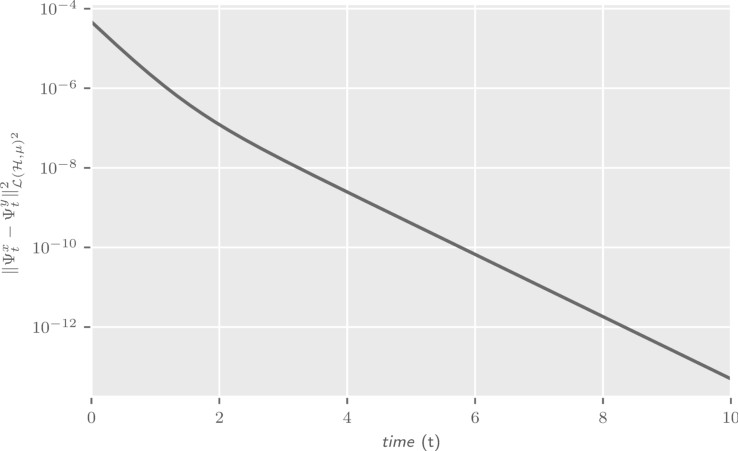
\includegraphics[width=\textwidth]{Fig3.pdf}
    \caption{
        $\mathcal{L}^2(\mathcal{H}, \mu)$
        distance between two solutions of the stochastic Fisher PDE
        with initial conditions $x = x(\xi)$, and  $y = \widehat{x}(\xi)$.
    }
    \label{fig:errorfisher}
\end{figure}

    \Cref{fig:likening_fisher_kpp} illustrates the distance between initial
conditions. The yellow pallet with transparency and a blue scale highlight the
zones where the two solutions are close. Thus, the zones where the color is
purple denotes, where the two solutions of SPDEs are close.
According to the $\mathcal{L}( \mathcal{H}, \mu)$-distance between the two
underlying solutions, \Cref{fig:errorfisher} confirms the above argument.

%
\subsection*{Stochastic Burgers equation}
Let $\mathcal{H} = L^2(0,1)$, consider the stochastic Burgers equation in the
interval $[0, 1]$
\begin{equation}
    \label{eqn:stochastic_burgers}
    \begin{aligned}
        d X(t, \xi) &=
            \left[
                \nu \partial_{\xi} ^ 2 X(t, \xi)
                + \frac{1}{2} \partial_{\xi} X^2(t, \xi)
            \right]dt
            +dW(t, \xi),
            \\
        X(t, 0) &= X(t, 1) =0, \quad t>0, \\
        X(0, \xi) &= x(\xi), \quad x\in \mathcal{H} \ .
    \end{aligned}
\end{equation}
As in the above experiment, we use the initial conditions
$x(\xi)$ and its truncated Chebyshev expansion
\begin{equation}
    x(\xi) := \sin(\pi \xi),
    \qquad
    \widehat{x}(\xi) :=
        \sum_{k=0} ^ N
         T_k x(\xi).
\end{equation}

\Cref{fig:approximationt0,fig:likening_burgers,fig:error_convergence}
illustrate a similar argument presented  in the above experiment.
\begin{figure}[htb]
    \caption{
        Numerical Solution of the Burgers
        \cref{eqn:stochastic_burgers}
        with initial conditions $x(\xi)$, $\widehat{x}(\xi)$.
     }
    \label{fig:approximationt0}
    \includegraphics[width=\linewidth, keepaspectratio]%
    {Fig4.pdf}
\end{figure}

\begin{figure}[htb]
    
    \centering
    \caption{
        Likening between two solution with closed
        initial conditions $x(\xi)$, and $\widehat{x}(\xi)$
        of the stochastic Burgers
        \cref{eqn:stochastic_burgers}.
        See \cite{plotlyFisher} to obtain other camera perspectives.
     }
    \label{fig:likening_burgers}
    \includegraphics[width=.9\textwidth, keepaspectratio]%
    {Fig5.pdf}
\end{figure}
%
\begin{figure}[htb]
    \centering
    \caption{
        Distance between two solutions of the
        stochastic Burgers
        \cref{eqn:stochastic_burgers}
        with initial conditions  $x = x(\xi)$, and $y = \widehat{x}(\xi)$.
     }
    \label{fig:error_convergence}
    \includegraphics[width=\linewidth, keepaspectratio]%
    {Fig6.pdf}
\end{figure}
\FloatBarrier
\section{Conclusions}
        To the best of our knowledge, our results represent the first
    contribution to the numeric stability respect to initial conditions of weak
    approximations of Kolmogorov equations in infinite dimensions. This kind of
    stability, combining with the weak approximation approach,
    would save computation time. That is, since our scheme asks specific
    conditions to obtain a weak numerical solution of an underlying SPDE, we
    convert the stochastic problem into a deterministic ODE for the first
    moment. This procedure overcome Montecarlo type simulations to  approximate
    moments or distributions\textemdash simulate many realization of the
    numerical stochastic process to approximate distributions or moments.
    Further, under  our setting, the regarding spectral approximation assures
    high precision and order of convergence. Thus we guess
    that our method would improve the time and save resources of
    computation. We are preparing another article to confirm this
    conjectures.

%\bibliographystyle{plainnat}
%\bibliography{references.bib}
\begin{thebibliography}{20}
\providecommand{\natexlab}[1]{#1}
\providecommand{\url}[1]{\texttt{#1}}
\expandafter\ifx\csname urlstyle\endcsname\relax
  \providecommand{\doi}[1]{doi: #1}\else
  \providecommand{\doi}{doi: \begingroup \urlstyle{rm}\Url}\fi

\bibitem[Barbu and Prato(2008)]{ba-da}
Viorel Barbu and Giuseppe~Da Prato.
\newblock {The Kolmogorov equation for a 2D-Navier–Stokes stochastic flow in
  a channel}.
\newblock \emph{Nonlinear Analysis: Theory, Methods \& Applications},
  69\penalty0 (3):\penalty0 940–949, 2008.
\newblock ISSN 0362-546X.
\newblock \doi{10.1016/j.na.2008.02.072}.
\newblock URL
  \url{http://www.sciencedirect.com/science/article/pii/S0362546X08001569}.
\newblock Trends in Nonlinear Analysis: in Honour of Professor
  V.Lakshmikantham.

\bibitem[Bogachev et~al.(2011)Bogachev, Prato, and R\"{o}ckner]{bo-da-ro}
Vladimir Bogachev, Giuseppe~Da Prato, and Michael R\"{o}ckner.
\newblock Existence results for fokker–planck equations in hilbert spaces.
\newblock In Robert Dalang, Marco Dozzi, and Francesco Russo, editors,
  \emph{Seminar on Stochastic Analysis, Random Fields and Applications VI},
  page 23–35, Basel, 2011. Springer Basel.
\newblock ISBN 978-3-0348-0021-1.

\bibitem[Chow(2007)]{liu}
Pao-Liu Chow.
\newblock \emph{Stochastic partial differential equations}.
\newblock Chapman \& Hall/CRC Applied Mathematics and Nonlinear Science Series.
  Chapman \& Hall/CRC, Boca Raton, FL, 2007.
\newblock ISBN 978-1-58488-443-9; 1-58488-443-6.

\bibitem[Da~Prato et~al.(2013)Da~Prato, Flandoli, and R\"{o}ckner]{da-fl-ro}
G.~Da~Prato, F.~Flandoli, and M.~R\"{o}ckner.
\newblock Fokker-planck equations for spde with non-trace-class noise.
\newblock \emph{Commun. Math. Stat.}, 1\penalty0 (3):\penalty0 281--304, 2013.
\newblock ISSN 2194-6701.
\newblock \doi{10.1007/s40304-013-0015-5}.
\newblock URL \url{https://doi.org/10.1007/s40304-013-0015-5}.

\bibitem[Da~Prato(2004)]{da}
Giuseppe Da~Prato.
\newblock \emph{Kolmogorov equations for stochastic {PDE}s}.
\newblock Advanced Courses in Mathematics. CRM Barcelona. Birkh\"{a}user
  Verlag, Basel, 2004.
\newblock ISBN 3-7643-7216-8.
\newblock \doi{10.1007/978-3-0348-7909-5}.
\newblock URL \url{https://doi.org/10.1007/978-3-0348-7909-5}.

\bibitem[{Da Prato} and Debussche(2007)]{da-de}
Giuseppe {Da Prato} and Arnaud Debussche.
\newblock {m-Dissipativity of Kolmogorov Operators Corresponding to Burgers
  Equations with Space-time White Noise}.
\newblock \emph{Potential Analysis}, 26\penalty0 (1):\penalty0 31–55, Feb
  2007.
\newblock ISSN 1572-929X.
\newblock \doi{10.1007/s11118-006-9021-5}.
\newblock URL \url{https://doi.org/10.1007/s11118-006-9021-5}.

\bibitem[Da~Prato and Zabczyk(1992)]{da-za1}
Giuseppe Da~Prato and Jerzy Zabczyk.
\newblock \emph{Stochastic equations in infinite dimensions}, volume~44 of
  \emph{Encyclopedia of Mathematics and its Applications}.
\newblock Cambridge University Press, Cambridge, 1992.
\newblock ISBN 0-521-38529-6.
\newblock \doi{10.1017/CBO9780511666223}.
\newblock URL \url{https://doi.org/10.1017/CBO9780511666223}.

\bibitem[Da~Prato and Zabczyk(2002)]{da-za}
Giuseppe Da~Prato and Jerzy Zabczyk.
\newblock \emph{Second order partial differential equations in {H}ilbert
  spaces}, volume 293 of \emph{London Mathematical Society Lecture Note
  Series}.
\newblock Cambridge University Press, Cambridge, 2002.
\newblock ISBN 0-521-77729-1.
\newblock \doi{10.1017/CBO9780511543210}.
\newblock URL \url{https://doi.org/10.1017/CBO9780511543210}.

\bibitem[Delgado-Vences and Flandoli(2016)]{de-fl}
Francisco Delgado-Vences and Franco Flandoli.
\newblock A spectral-based numerical method for {K}olmogorov equations in
  {H}ilbert spaces.
\newblock \emph{Infin. Dimens. Anal. Quantum Probab. Relat. Top.}, 19\penalty0
  (3):\penalty0 1650020, 37, 2016.
\newblock ISSN 0219-0257.
\newblock \doi{10.1142/S021902571650020X}.
\newblock URL \url{https://doi.org/10.1142/S021902571650020X}.

\bibitem[Diaz-Infante({\natexlab{a}})]{plotlyBurgers}
Saul Diaz-Infante.
\newblock Likening of two solutions of the burgers equation with two initial
  function conditions.
\newblock https://plot.ly/~sauldiazinfante/30/ [2019/05/11], {\natexlab{a}}.
\newblock URL \url{https://plot.ly/~sauldiazinfante/30/}.

\bibitem[Diaz-Infante({\natexlab{b}})]{plotlyFisher}
Saul Diaz-Infante.
\newblock Likening of two solutions of the fisher equation with two initial
  function conditions.
\newblock https://plot.ly/~sauldiazinfante/28/ [2019/05/11], {\natexlab{b}}.
\newblock URL \url{https://plot.ly/~sauldiazinfante/28/}.

\bibitem[Gottlieb et~al.(1987)Gottlieb, Lustman, and Tadmor]{Gottlieb1987a}
David Gottlieb, Liviu Lustman, and Eitan Tadmor.
\newblock Stability analysis of spectral methods for hyperbolic
  initial-boundary value systems.
\newblock \emph{SIAM J. Numer. Anal.}, 24\penalty0 (2):\penalty0 241--256,
  1987.
\newblock ISSN 0036-1429.
\newblock \doi{10.1137/0724020}.
\newblock URL \url{https://doi.org/10.1137/0724020}.

\bibitem[Imkeller(2008)]{im}
Peter Imkeller.
\newblock \emph{Malliavin's calculus and applications in stochastic control and
  finance}, volume~1 of \emph{IMPAN Lecture Notes}.
\newblock Polish Academy of Sciences, Institute of Mathematics, Warsaw, 2008.
\newblock ISBN 978-83-86806-02-7.

\bibitem[Lang et~al.(2017)Lang, Petersson, and Thalhammer]{Lang2017}
Annika Lang, Andreas Petersson, and Andreas Thalhammer.
\newblock {Mean-square stability analysis of approximations of stochastic
  differential equations in infinite dimensions}.
\newblock \emph{BIT Numerical Mathematics}, 57\penalty0 (4):\penalty0
  963–990, Dec 2017.
\newblock ISSN 1572-9125.
\newblock \doi{10.1007/s10543-017-0684-7}.
\newblock URL \url{https://doi.org/10.1007/s10543-017-0684-7}.

\bibitem[Li et~al.(2019)Li, Fiordilino, and Feng]{Li2019}
Ning Li, Joseph Fiordilino, and Xinlong Feng.
\newblock {Ensemble Time-Stepping Algorithm for the Convection-Diffusion
  Equation with Random Diffusivity}.
\newblock \emph{Journal of Scientific Computing}, 79\penalty0 (2):\penalty0
  1271--1293, May 2019.
\newblock ISSN 1573-7691.
\newblock \doi{10.1007/s10915-018-0890-8}.
\newblock URL \url{https://doi.org/10.1007/s10915-018-0890-8}.

\bibitem[Matzumiya(2019)]{matsumyaRepo}
Alan~Daniel Matzumiya.
\newblock Github of the python implementation of the weak spectral method.
\newblock \url{https://github.com/alanmatzumiya/Paper}, May 2019.
\newblock URL \url{https://github.com/alanmatzumiya/Paper}.

\bibitem[Milstein and Tretyakov(2013)]{milstein2013stochastic}
Grigori~Noah Milstein and Michael~V Tretyakov.
\newblock \emph{Stochastic numerics for mathematical physics}.
\newblock Springer Science \& Business Media, 2013.

\bibitem[Schwab and S{\"u}li(2013)]{schwab2013adaptive}
Christoph Schwab and Endre S{\"u}li.
\newblock Adaptive galerkin approximation algorithms for kolmogorov equations
  in infinite dimensions.
\newblock \emph{Stochastic Partial Differential Equations: Analysis and
  Computations}, 1\penalty0 (1):\penalty0 204--239, 2013.

\bibitem[Trefethen and Trummer(1987)]{Trefethen1987}
Lloyd~N. Trefethen and Manfred~R. Trummer.
\newblock An instability phenomenon in spectral methods.
\newblock \emph{SIAM J. Numer. Anal.}, 24\penalty0 (5):\penalty0 1008--1023,
  1987.
\newblock ISSN 0036-1429.
\newblock \doi{10.1137/0724066}.
\newblock URL \url{https://doi.org/10.1137/0724066}.

\bibitem[Zhang and Karniadakis(2017)]{zhang2017numerical}
Zhongqiang Zhang and George Karniadakis.
\newblock \emph{Numerical methods for stochastic partial differential equations
  with white noise}.
\newblock Springer, 2017.

\end{thebibliography}
\end{document}
